\section{\large Конструкторская часть}

Конструкторская часть проектирования базы данных включает в себя несколько этапов, начиная от анализа требований и разработки концептуальной модели, заканчивая созданием физического дизайна БД. Один из самых важных этапов --- это определение правил и триггеров, которые должны контролировать целостность данных в базе и предоставляют широкую возможность модификации базы данных.

\subsection{Формализация сущностей системы}

При проектировании базы данных необходимо определить все сущности, которые будут использоваться в системе. Каждая сущность представляет собой объект, который имеет свои атрибуты и отношения с другими сущностями. 

На основе выделенных ранее сущностей \ref{fig:anal:use-case} спроектированы таблицы 
базы данных, где содержаться название полей, которые будут представлены в базе данных.

\subsubsection{Таблица Visitor}

Содержит информацию о посетителях магазинов, которые включает следующие поля:

\begin{enumerate}[label=\arabic*.]
    \item id --- индетификатор пользователя, который является первичным ключом;
    \item description --- описание пользователя, вещественный тип;
    \item location --- положение пользователя на плане магазина, символьный тип 
    который состои из двух вещественных чисел;
    \item view --- вектор взгляда, символьный тип, состоящий из шести вещественных
    чисел, которые задают вектор взгляда;
    \item detection --- описание пользователя, символьный тип, 
    состоящий из 4 вещественных
    чисел, которые задают прямоугольник обнаружения посетителя.
\end{enumerate}

\subsubsection{\large Таблица Camera}

Содержит информацию о камерах в магазине, которые включает следующая поля:

\begin{enumerate}[label=\arabic*.]
    \item id --- номер камеры в магазине, первичный ключ;
    \item location --- положение пользователя на плане магазина, символьный тип 
    который состои из трех вещественных чисел;
    \item resolution --- разрешение камеры, символьный тип состоящий из двух
    вещественных чисел;
    \item rotation --- наклон камеры, символьный тип. Является матрицей
    состоящих из 9 вещественных чисел;
    \item type --- тип камеры, символьный тип.
\end{enumerate}

\subsubsection{Таблица Shelf}

Таблица полок необходима для представления местоположения товаров, и дает представление с какими товарами взаимодействуют посетители магазина. Она содержит информацию о полках с товарами в магазине, которые включает следующая поля:

\begin{enumerate}[label=\arabic*.]
    \item id --- номер полки в магазине, первичный ключ;
    \item location --- положение пользователя на плане магазина, символьный тип 
    который состои из трех вещественных чисел;
    \item length --- длина полки, вещественный тип.
\end{enumerate}

\subsubsection{Таблица Product}

Таблица продуктов необходима для представления товаров в магазине, данная информация поможет структурировать доходы и расходы магазинов.
Она содержит информацию о товарах в магазине, которые включает следующая поля:

\begin{enumerate}[label=\arabic*.]
    \item id --- номер товара в магазине, первичный ключ;
    \item location --- положение товара на плане магазина, символьный тип 
    который состои из трех вещественных чисел;
    \item name --- имя товара, символьный тип;
    \item dataEnd --- срок годности, тип дата;
    \item weight --- вес товара, вещественный тип;
    \item status --- статус товара, целочисленный тип;
    \item price --- цена товара, вещественный тип.
\end{enumerate}

\subsubsection{Таблица ChainStore}

Данная таблица объединяет разные магазины в одну общую таблицу, что позволит получать общую информацию сетей магазинов.
Она содержит информацию о сетях магазинов, которые включает следующая поля:

\begin{enumerate}[label=\arabic*.]
    \item id --- номер магазина, первичный ключ;
    \item location --- положение магазина в городе, символьный тип 
    который состои из двух вещественных чисел (широта и долгота);
    \item name --- имя магазина, символьный тип;
    \item nameDir --- имя директора магазина, символьный тип;
    \item income --- доход магазина, вещественный тип;
    \item consumption --- расходы магазина, вещественный тип.
\end{enumerate}

% На рисунке \ref{fig:cons:ER} предствалена ER диаграмма база данных.

%\begin{figure}[ht!]
%	\centering
%	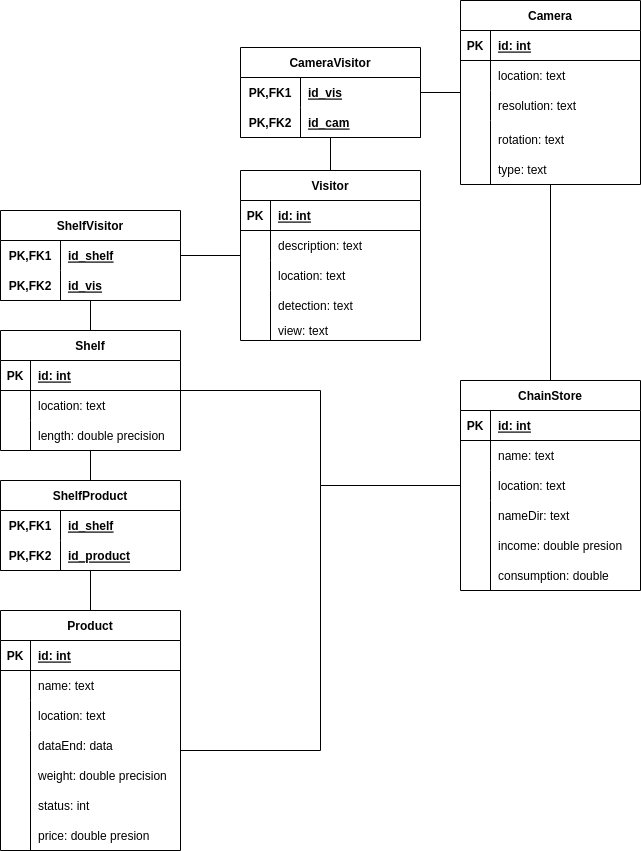
\includegraphics[width=0.55\linewidth]{assets/images/ER-diagram.drawio.png}
%	\caption{Use-case диаграмма}
%	\label{fig:cons:ER}
%\end{figure}
%\FloatBarrier

\subsection{Ролевая модель}

Для эффективного взаимодействия пользователей с системой управления базами данных была разработана ролевая модель, которая позволит определить доступные функциональные возможности каждому пользователю в соответствии с его ролями и ответственностями. Это значительно повышает безопасность и защищенность системы, так как пользователи не имеют доступа к чувствительным данным, которые не относятся к их компетенции.

Кроме того, ролевая модель облегчает работу администраторов, так как она позволяет быстро и удобно настраивать доступ к базам данных для конкретных пользователей или групп пользователей. Также благодаря ролевой модели упрощается процесс мониторинга и аудита действий пользователей в системе.

Таким образом, ролевая модель является важной составляющей системы управления базами данных, которая обеспечивает ее надежную и бесперебойную работу в соответствии с требованиями пользователям и бизнес-процессам.

\subsubsection{Сотрудник Employee}

В данном случае, роль пользователей имеет право выполнения операции SELECT над таблицей Visitor.

Операция SELECT позволяет выбирать данные из указанной таблицы. В данном случае, роль имеет доступ только к таблице Visitor и может выбирать из нее информацию, но не может изменять, удалять или добавлять новые данные.

Такая ролевая модель может быть полезна для обеспечения безопасности данных в системе управления базами данных (СУБД). Она позволяет ограничить доступ пользователей к чувствительным данным и установить строгий контроль за использованием данных.

\begin{enumerate}[label=\arabic*.]
    \item SELECT --- над таблицей Visitor.
\end{enumerate}


\subsubsection{Охрана Security}

Это описание также относится к ролевой модели управления доступом к данным в базе данных. Роль пользователей, которой предоставлены данные привилегии, имеет право выполнения операции SELECT над таблицами Visitor, Camera, Product и Shelf.

Таким образом, данная роль имеет более широкий доступ к данным, чем в предыдущем описании. Она может выбирать информацию из четырех таблиц: Visitor, Camera, Product и Shelf. Операция SELECT позволяет выбирать данные из указанных таблиц, но не изменять или удалять их.


\begin{enumerate}[label=\arabic*.]
    \item SELECT --- над таблицей Visitor;
    \item SELECT --- над таблицами Camera, Product, Shelf.
\end{enumerate}


\subsubsection{Администратор Administrator}

Роль администратора имеет полный доступ ко всем таблицам в базе данных и обладает всеми правами на выполнение операций с данными.

\begin{enumerate}[label=\arabic*.]
    \item все права над таблицами Visitor;
    \item все права над таблицами Camera, Product, Shelf;
    \item все права над таблицами ChainStore.
\end{enumerate}

Таким образом, администратор - это самый привилегированный пользователь в системе управления базами данных. Ему предоставляется полный контроль над всеми аспектами работы с данными в базе данных и он может выполнять любые необходимые операции.

% Ролевая модель на уровне СУБД позволяет обеспечить безопасное управление данными.

\subsection{Разработка триггера и функции}

В СУБД предусмотрена функция, которая проверяет местоположение пользователя относительно выхода. 
Данная функция возвращает статус посетителя (находится внутри или вне магазина).

Также системе представлен ALTER триггер, который оповещает систему о том, 
что посетитель вышел из магазина.


\subsection*{Вывод}

В данном разделе были формализированны сущности системы, представлен рисунок диаграммы сущности системы,
выделены ролевые модели, спроектированы триггер и функция.